\documentclass{beamer}
\usetheme{Madrid}
\usepackage{tikz}

\newcommand{\F}{\mathbb{F}}
\newcommand{\B}{\mathcal B}
\newcommand{\HH}{\mathcal H}
\newcommand{\RR}{\mathcal R}
\newcommand{\cl}{\operatorname{cl}}
\newcommand{\si}{\operatorname{si}}
\newcommand{\PG}{\operatorname{PG}}
\newcommand{\Aut}{\operatorname{Aut}}

\title[Quinary excluded minors]{Rank-four, eleven-element excluded minors for representability over \texorpdfstring{$\F_5$}{GF(5)}}
\author{Anonymous}
\date{2026}

\begin{document}

\frame{\titlepage}

\begin{frame}
  \frametitle{Basic concepts}
  \begin{itemize}
    \item A \emph{matroid} consists of a finite ground set $E$ and a family
      $\mathcal I$ of \emph{independent sets} that obeys three axioms.
      \begin{itemize}
        \item $\varnothing\in\mathcal I$.
        \item Every subset of an independent set is independent.
        \item If $I,J\in\mathcal I$ and $|I|<|J|$, then some
          $j\in J\setminus I$ makes $I\cup\{j\}$ independent.
      \end{itemize}
    \item In a \emph{vector matroid}, the elements label the columns of a
      matrix. A set is independent exactly when its columns are linearly
      independent.
    \item A matroid is \emph{$\F$-representable} if some matrix over the
      field $\F$ realizes its independent sets in this way.
  \end{itemize}
\end{frame}

\begin{frame}
  \frametitle{Bases, duality and minors}
  \begin{itemize}
    \item A \emph{basis} is a maximal independent set. All bases have the
      same size, the \emph{rank}. The ground set and the bases determine
      the matroid.
    \item For example, the columns labelled $0,1,2$ of
      $\left(\begin{smallmatrix}1&1&0\\0&0&1\end{smallmatrix}\right)$
      give the bases $\{\{1,2\},\{0,2\}\}$.
    \item The \emph{dual} $M^*$ has the same ground set as $M$ and bases
      $\{E\setminus B:B\in\B(M)\}$.
    \item A \emph{minor} is obtained by deletions and contractions.
      \begin{itemize}
        \item Deletion $M\setminus T$ keeps the independent sets disjoint
          from $T$. For a vector matroid, delete the columns in $T$.
        \item Contraction is $M/T=(M^*\setminus T)^*$. For a vector
          matroid, quotient by the span of the columns in $T$ and keep
          the remaining columns.
      \end{itemize}
  \end{itemize}
\end{frame}

\begin{frame}
  \frametitle{Problem statement}
  \begin{itemize}
    \item A matroid is \emph{quinary} if it is representable over
      $\F_5=\mathbb Z/5\mathbb Z$.
    \item An \emph{excluded minor} for quinary representability is a
      nonquinary matroid all of whose proper minors are quinary.
    \item It suffices to check $M/a$ and $M\setminus a$ for every
      $a\in E(M)$, since representability is preserved under taking minors.
  \end{itemize}
  \begin{block}{Classification}
    There are exactly \textbf{35 isomorphism classes} of rank-four,
    eleven-element excluded minors for quinary representability.
  \end{block}
\end{frame}

\begin{frame}
  \frametitle{LLM-assisted computation}
  \begin{itemize}
    \item A direct prompt left the classification incomplete. We used
      an LLM with computational tools to develop and carry out the search.
    \item The proof reduces the classification to a finite search that
      enumerates all candidates. SageMath handles exact isomorphism
      checks, and natural joins combine compatible deletion data.
    \item We checked separate certificates for nonrepresentability and
      for the immediate minors of every final matroid.
  \end{itemize}
\end{frame}

\begin{frame}
  \frametitle{Proof outline}
  View an eleven-element excluded minor $M$ as an extension of a
  ten-element quinary \emph{parent} $N=M\setminus e$.
  \begin{enumerate}
    \item Generate all possible parents $N$ up to isomorphism.
    \item For each $N$, recover all nonquinary extensions $M$ whose
      deletions are quinary. For $f\in E(N)$, obtain possible
      $M\setminus f$ by extending $N\setminus f$ by $e$.
    \item Test all single-element contractions of each candidate and
      remove isomorphic repeats.
  \end{enumerate}
\end{frame}

\begin{frame}
  \frametitle{Step 1: generating parents}
  Every parent is connected and simple of rank four. Simplicity
  rules out loops and parallel pairs.

  \medskip
  Matrices over $\F_5$ are \emph{field-isomorphic} if they differ by
  invertible row operations, nonzero column scalings and a column
  permutation.
  \begin{itemize}
    \item Any basis can be reduced to $I_4$, so start with $I_4$.
      At each size, append every unused projective point (one nonzero
      vector per one-dimensional subspace). Use Sage to retain one
      matrix per field-isomorphism class.
    \item Convert the ten-column matrices to basis families, deduplicate
      up to matroid isomorphism and keep the connected parents.
    \item Keep the matrix catalogue separately. One matroid can have
      several field-isomorphism classes of representations.
  \end{itemize}
\end{frame}

\begin{frame}
  \frametitle{Step 2: labelled extensions}
  Fix the parent labels $P=\{0,\ldots,9\}$ and the new label $e=10$.
  Let $\mathcal P$ contain one labelled representative of each
  connected simple rank-four quinary matroid on ten elements.

  \medskip
  For each $N\in\mathcal P$, let $\mathcal D(N)$ be the set of simple
  rank-four matroids $M$ on $P\cup\{e\}$ such that
  \begin{itemize}
    \item $M\setminus e=N$,
    \item $M$ is nonquinary, and
    \item $M\setminus a$ is quinary for every $a\in P\cup\{e\}$.
  \end{itemize}
  We keep the labels fixed until the final isomorphism checks.
  Each $N\setminus f$ still has rank four because $N$ is connected.
\end{frame}

\begin{frame}
  \frametitle{Step 2: compatibility of deletions}
  The bases avoiding $e$ are fixed by $N$. For each triple $T\subseteq P$,
  let $x_T$ record whether $T\cup\{e\}$ is a basis. Let $\pi_f(x)$ keep
  the bits for triples avoiding $f$.

  \medskip
  For $Q=N$ or $N\setminus f$, let $\RR(Q)$ contain the bit rows on
  triples of $E(Q)$ for all simple rank-four quinary extensions by $e$.
  \begin{itemize}
    \item $x\in\RR(N)$ gives a quinary extension of $N$.
    \item $\pi_f(x)\in\RR(N\setminus f)$ gives a quinary deletion at $f$.
  \end{itemize}

  \textbf{Key fact.} If the proposed bases avoiding each element define
  a simple rank-four matroid, the full family defines one too.
  Any two bases use at most eight of the eleven elements, so basis
  exchange can be checked in a common deletion. Each pair of elements
  also survives in some simple deletion.
  \[
    \mathcal S(N)=
    \{x:\pi_f(x)\in\RR(N\setminus f)\text{ for every }f\in P\}
    \setminus\RR(N).
  \]
  These rows correspond bijectively to $\mathcal D(N)$.
\end{frame}

\begin{frame}
  \frametitle{Step 2.1: labelled representations}
  For $Q=N$ or $N\setminus f$, a \emph{labelled representation} of
  $Q$ is a matrix over $\F_5$ whose columns carry the element labels
  of $Q$ and realize its bases.

  \medskip
  Two such matrices are \emph{labelled projectively equivalent}
  if row operations and nonzero column scalings relate them with
  labels fixed. We build $\mathcal L(Q)$ with one matrix per class.
  \begin{enumerate}
    \item Take one matrix from each field-isomorphism class whose
      matroid is isomorphic to $Q$. Align its labels with $Q$ using
      one matroid isomorphism.
    \item Apply the automorphisms of $Q$ to these column labels to
      reach all other alignments.
    \item Normalize the resulting matrices and keep the distinct ones.
  \end{enumerate}
\end{frame}

\begin{frame}
  \frametitle{Step 2.1: computing automorphisms}
  Build a coloured bipartite incidence graph for $Q$.
  \begin{itemize}
    \item Use a blue vertex for each element and a red vertex for each
      basis.
    \item Connect an element vertex to a basis vertex exactly when the
      element belongs to the basis.
    \item The colour-preserving graph automorphisms induce exactly
      $\Aut(Q)$ on the element vertices.
  \end{itemize}
  Sage supplies generators of this group. Repeatedly apply the
  generators and keep each new normalized matrix to exhaust the orbit.
\end{frame}

\begin{frame}
  \frametitle{Step 2.1: normalizing matrices}
  Fix an ordered basis $B=(b_1,\ldots,b_r)$ of $Q$. Reduce its
  columns to $I_r$ by Gaussian elimination and write the remaining
  block as $Z$. The bases of $Q$ determine the support of $Z$.
  \[
    Z_{ij}\ne0
    \quad\Longleftrightarrow\quad
    (B\setminus\{b_i\})\cup\{j\}\in\B(Q).
  \]
  Equivalent reduced blocks differ only by row and column scalings.
  \begin{itemize}
    \item Form the bipartite graph of rows and columns of $Z$, with
      an edge for each nonzero entry.
    \item Fix a spanning forest. In each tree, start with a root
      multiplier of $1$ and choose the remaining multipliers so
      every tree entry becomes $1$.
    \item The resulting block is unique for the equivalence class.
      Any further scalings that preserve the tree entries cancel
      on every edge of that component.
  \end{itemize}
\end{frame}

\begin{frame}
  \frametitle{Step 2.2: building the extension tables}
  For each $V\in\mathcal L(Q)$, append each unused point $v$ of
  $\PG(3,5)$ as column $e$. The matrix $[V\mid v]$ represents a
  simple rank-four quinary extension of $Q$. Its row is
  \[
    z(V,v)_T=\mathbf 1\!\left\{\det[\,V_T\mid v\,]\ne 0\right\},
    \qquad T\in\binom{E(Q)}{3}.
  \]
  The distinct rows obtained this way are exactly $\RR(Q)$.

  \medskip
  \textbf{Batching the determinant tests.}
  For each triple, expand along $v$ to write the determinant as
  $c_T^{\mathsf T}v$. Stack the cofactor rows in $C$ and the $156$
  projective point columns in $D$. The product $CD$ over $\F_5$
  gives all tests for this $V$ at once.
\end{frame}

\begin{frame}
  \frametitle{Step 2.3: compressing the tables}
  Dependent triples always give bit $0$. Independent triples
  spanning the same rank-three flat (hyperplane) $H$ have the same
  bit $y_H$, since they span $e$ exactly when $H$ does.

  \medskip
  Let $\HH(N)$ be the hyperplanes of $N$. The columns visible in
  the deletion of $f$ are
  \[
    C_f=\left\{\cl_N(T):T\in\binom{P\setminus\{f\}}{3},
                             \ r_N(T)=3\right\},
  \]
  where $\cl_N(T)$ is the set of elements spanned by $T$ in $N$.
  Compress $\RR(N\setminus f)$ to $A_f$ on $C_f$ and $\RR(N)$
  to $A$ on $\HH(N)$. The same solutions in hyperplane coordinates are
  \[
    \widehat{\mathcal S}(N)=
    \{y\in\{0,1\}^{\HH(N)}:y|_{C_f}\in A_f
                   \text{ for every }f\in P\}\setminus A.
  \]
\end{frame}

\begin{frame}
  \frametitle{Step 2.4: natural join}
  \begin{itemize}
    \item As in a database join, combine two rows exactly when they
      agree on all shared columns.
    \item Join the deletion tables $A_f$ one at a time. Every
      hyperplane $H$ appears in a table, since deleting any
      $f\notin H$ leaves its spanning triples intact.
    \item Remove the full rows that appear in $A$. The remaining
      rows form $\widehat{\mathcal S}(N)$.
  \end{itemize}
  \[
    \widehat{\mathcal S}(N)=(A_0\Join\cdots\Join A_9)\setminus A.
  \]
  The eleven-element search used this method for every connected parent.
\end{frame}

\begin{frame}
  \frametitle{Step 2.4: SAT enumeration}
  Use one Boolean variable $y_H$ per hyperplane.
  \begin{columns}[T,onlytextwidth]
    \begin{column}{0.60\textwidth}
      \begin{enumerate}
        \item Encode each $A_f$ as a binary decision diagram and
          require its root to accept.
        \item Block each row of $A$.
        \item Record and block each solution until UNSAT.
      \end{enumerate}
    \end{column}
    \begin{column}{0.37\textwidth}
      \centering
      \small Example table $\{00,01,11\}$

      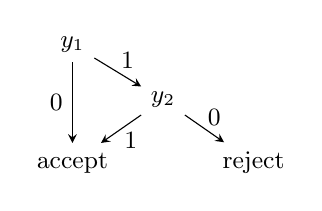
\begin{tikzpicture}[>=stealth,every node/.style={font=\small}]
        \node (first) at (0,0) {$y_1$};
        \node (second) at (1.15,-0.70) {$y_2$};
        \node (accept) at (0,-1.50) {accept};
        \node (reject) at (2.30,-1.50) {reject};
        \draw[->] (first) -- node[left] {$0$} (accept);
        \draw[->] (first) -- node[above right,inner sep=1pt] {$1$} (second);
        \draw[->] (second) -- node[below right,inner sep=1pt] {$1$} (accept);
        \draw[->] (second) -- node[above right,inner sep=1pt] {$0$} (reject);
      \end{tikzpicture}
    \end{column}
  \end{columns}

  \medskip
  At a node testing $y_H$, let $v$ be its value and $\ell,h$ the
  values of its $0,1$ branches. Its equivalence and four clauses are
  \[
    \begin{gathered}
      v\leftrightarrow((\neg y_H\land\ell)\lor(y_H\land h))\\[3pt]
      (\neg v\lor y_H\lor\ell),\qquad(\neg v\lor\neg y_H\lor h),\\
      (v\lor y_H\lor\neg\ell),\qquad(v\lor\neg y_H\lor\neg h).
    \end{gathered}
  \]
  To block row $a$, add $\bigvee_{H\in\HH(N)}(y_H\ne a_H)$.
  SAT cross-checked the joins at nine and ten elements.
\end{frame}

\begin{frame}
  \frametitle{Step 3: testing contractions}
  For each $M\in\mathcal D(N)$ and each $a\in E(M)$, test
  $M/a$ for quinary representability.
  \begin{itemize}
    \item Each single-element contraction has rank three because
      $M$ is simple of rank four.
    \item Simplify $M/a$ by deleting loops and keeping one element from
      each parallel class. A representation of $\si(M/a)$ can restore
      the removed elements as zero columns or parallel copies.
    \item Compare each simplification with the complete rank-three
      quinary catalogue generated by the same method as in Step~1.
    \item Keep the candidates that pass every test and use Sage to
      deduplicate them up to isomorphism.
  \end{itemize}
\end{frame}

\begin{frame}
  \frametitle{Search results and certificates}
  \begin{center}
    \begin{tabular}{lr}
      \textbf{Stage} & \textbf{Count} \\
      \hline
      Simple ten-element parent classes & $58{,}756$ \\
      Connected parent classes in $\mathcal P$ & $58{,}672$ \\
      Labelled pairs $(N,M)$ with $M\in\mathcal D(N)$ & $659$ \\
      Classes after contraction tests and deduplication & $\mathbf{35}$
    \end{tabular}
  \end{center}
  We verified each final representative independently.
  \begin{itemize}
    \item A checked DRAT refutation proves the determinant constraints
      for a representing matrix are unsatisfiable.
    \item We checked $22$ matrices witnessing representability of its
      deletions and contractions.
  \end{itemize}
  A separate incidence-graph check verified pairwise nonisomorphism.
\end{frame}

\begin{frame}
  \frametitle{Future work}
  Complete the classification on eleven elements.
  \begin{itemize}
    \item Duality pairs rank $r$ with rank $11-r$, so the rank-four
      classification also gives the rank-seven classification.
    \item Existing classifications cover ranks up to three.
      Up to duality, rank five is the remaining case.
    \item The deletion-compatibility argument still applies at rank
      five, since $11>2\cdot5$.
  \end{itemize}
  \smallskip
  {\footnotesize
   \href{https://matroidunion.org/?p=3244}{Campbell (2020), \emph{The rank-3 excluded minors for GF(5)-representability}}}
\end{frame}

\end{document}
